\documentclass{article}
\usepackage{graphicx}
\usepackage{amsmath}
\usepackage{geometry}
\geometry{letterpaper, portrait, margin=1in}
\usepackage{listings}
\usepackage{color}

\definecolor{mygreen}{rgb}{0,0.6,0}
\definecolor{mygray}{rgb}{0.5,0.5,0.5}
\definecolor{mymauve}{rgb}{0.58,0,0.82}

\lstset{
  backgroundcolor=\color{white},
  basicstyle=\footnotesize,
  breaklines=true,
  captionpos=b,
  commentstyle=\color{mygreen},
  escapeinside={\%*}{*)},
  keywordstyle=\color{blue},
  stringstyle=\color{mymauve},
  rulecolor=\color{black},
  numbers=left,
  numberstyle=\tiny\color{mygray},
  numbersep=5pt,
  showstringspaces=false,
  keepspaces=true,
}

\begin{document}

\title{ELCT 562 CA 1}
\author{Jacob Vaught}
\date{\today}
\maketitle

\section*{Executive Summary}
This document provides an analysis of wireless signal propagation characteristics over a range of distances for frequencies of 2.450 GHz and 5.450 GHz. The MATLAB script initializes constants for radio communications, calculates noise power, and prepares separate figures for path loss, RX power, SNR, and channel capacity. It plots these characteristics against distance, records values at 50 meters, and tabulates them. The script concludes by displaying the results in customized plots.

\section*{Mathematical Background}
The following equations are used in the analysis:

\begin{itemize}
    \item Noise Power in dBm:
    \begin{equation}
        P_{\text{noise}} = 10\log_{10}(kTB) + NF
    \end{equation}
    where $k$ is Boltzmann's constant, $T$ is the temperature, $B$ is the bandwidth, and $NF$ is the noise figure.

    \item Path Loss in dB:
    \begin{equation}
        PL = 20\log_{10}(d_0) + 20\log_{10}(f) - 147.55 + Gt + Gr + 10\gamma\log_{10}\left(\frac{d}{d_0}\right)
    \end{equation}
    where $d_0$ is the reference distance, $f$ is the frequency, $Gt$ and $Gr$ are transmit and receive antenna gains, $\gamma$ is the path loss exponent, and $d$ is the distance.

    \item Received Power (RX Power in dBm):
    \begin{equation}
        P_{\text{rx}} = P_t - PL
    \end{equation}
    where $P_t$ is the transmit power and $PL$ is the path loss.

    \item Signal-to-Noise Ratio (SNR in dB):
    \begin{equation}
        SNR_{\text{dB}} = P_{\text{rx}} - P_{\text{noise}}
    \end{equation}
    where $P_{\text{rx}}$ is the received power and $P_{\text{noise}}$ is the noise power.

    \item Channel Capacity in Mbit/s (Shannon's theorem):
    \begin{equation}
        C = \frac{B \cdot \log_2(1 + SNR_{\text{linear}})}{1e6}
    \end{equation}
    where $C$ is the channel capacity, $B$ is the bandwidth, and $SNR_{\text{linear}}$ is the SNR converted from dB to a linear scale.
\end{itemize}

\section*{Results and Discussion}
The following figures illustrate the characteristics of wireless channel versus distance for the given frequencies:

\begin{figure}[h!]
\centering

\includegraphics[width=0.7\textwidth]{RX.png}
\caption{Received Power vs. Distance: The plot shows a rapid decline in RX power over short distances, which then tapers off, indicating the initial strong influence of path loss.}
\end{figure}

\begin{figure}[h!]
\centering
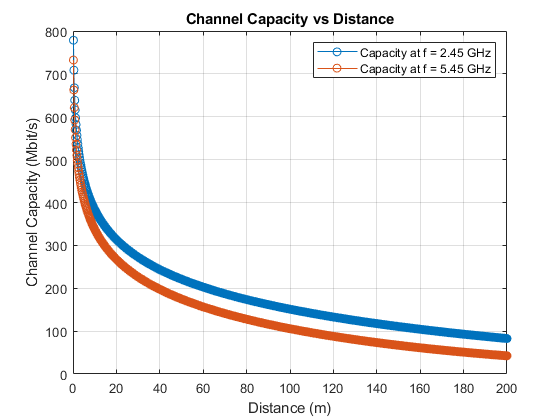
\includegraphics[width=0.7\textwidth]{CC.png}
\caption{Channel Capacity vs. Distance: Channel capacity reduces with distance, with a steep initial drop followed by a more gradual decline, mirroring the SNR trend.}
\end{figure}

\begin{figure}[h!]
\centering
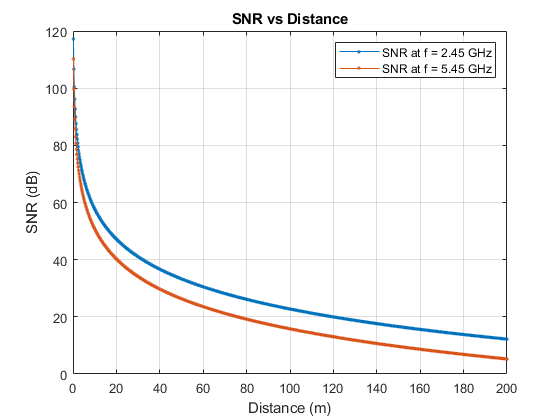
\includegraphics[width=0.7\textwidth]{SNR.png}
\caption{Signal-to-Noise Ratio vs. Distance: SNR decreases with distance, sharply at first and then at a slower rate, similar to the channel capacity plot but with different numerical values.}
\end{figure}

\begin{figure}[h!]
\centering
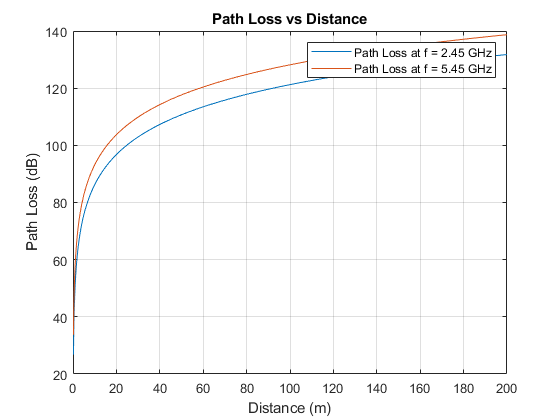
\includegraphics[width=0.7\textwidth]{PL.png}
\caption{Path Loss vs. Distance: This plot illustrates the increase in path loss with distance. The rate of increase is high initially, showing significant loss at shorter ranges, and gradually levels off, indicating less sensitivity to distance as the range increases.}
\end{figure}

The tabulated results at 50 meters provide a reference point to assess the quality of the communication link at a given distance. The analysis of the plots reveals the expected decrease in RX power and SNR with increasing distance, while path loss increases. The channel capacity also decreases as distance increases, which is consistent with Shannon's theorem.
\section*{Tabulated Results at 50 Meters}
Below are the tabulated results for the two frequencies at a distance of 50 meters:

\begin{table}[h]
\centering
\begin{tabular}{ccccc}
\toprule
Frequency (GHz) & Path Loss (dB) & RX Power (dBm) & SNR (dB) & Capacity (Mbps) \\
\midrule
2.45 & -110.71 & -90.712 & 33.252 & 220.94 \\
5.45 & -117.66 & -97.657 & 26.308 & 174.85 \\
\bottomrule
\end{tabular}
\caption{Comparison of signal characteristics at 50 meters for 2.45 GHz and 5.45 GHz frequencies.}
\end{table}
\newpage
\section*{MATLAB Code}
The following MATLAB code was used for generating the plots and analysis:

\begin{lstlisting}[language=Matlab]
% Clear the workspace and figures
clc
clear all
close all

% Define constants
c = 3e8; % Speed of light in m/s
Gt = 9; % Transmit antenna gain in dB
Gr = 2; % Receive antenna gain in dB
frequencies = [2.450e9, 5.450e9]; % Frequencies in Hz
d = linspace(0, 200, 1000); % Distance vector from 0 to 200 meters
d0 = 1; % Reference distance in meters
gamma = 3.5; % Path loss exponent
Pt = 20; % Transmit power in dBm
BW = 20e6; % Bandwidth in Hz
NF = 7; % Noise figure in dB
k = 1.38064852e-23; % Boltzmann constant in J/K
T = 290; % Standard temperature in Kelvin

% Calculate noise power (in dBm)
noise_power_dbm = 10*log10(k*T*BW) + NF;

% Initialize arrays to store results for tabulation
path_loss_at_50m = zeros(length(frequencies), 1);
Prx_at_50m = zeros(length(frequencies), 1);
SNR_db_at_50m = zeros(length(frequencies), 1);
capacity_at_50m = zeros(length(frequencies), 1);

% Initialize figures for each characteristic
figure_path_loss = figure;
figure_rx_power = figure;
figure_snr = figure;
figure_capacity = figure;

% Loop over the two frequencies
for i = 1:length(frequencies)
    f = frequencies(i);
    % Calculate path loss at reference distance
    Pfspl = 20*log10(d0)+20*log10(f)-147.55 + Gt + Gr;
    
    % Calculate path loss over the distances
    path_loss = Pfspl + 10*gamma*log10(d/d0);
    
    % Plot path loss
    figure(figure_path_loss);
    plot(d, path_loss, 'DisplayName', ['Path Loss at f = ' num2str(f/1e9) ' GHz']);
    hold on;
    
    % Calculate RX power over the distances
    Prx = Pt - path_loss;
    
    % Plot RX power
    figure(figure_rx_power);
    plot(d, Prx, '--', 'DisplayName', ['RX Power at f = ' num2str(f/1e9) ' GHz']);
    hold on;
    
    % Calculate SNR over the distances
    SNR_db = Prx - noise_power_dbm;
    
    % Plot SNR
    figure(figure_snr);
    plot(d, SNR_db, '.-', 'DisplayName', ['SNR at f = ' num2str(f/1e9) ' GHz']);
    hold on;
    
    % Calculate channel capacity (Shannon's theorem) over the distances
    SNR_linear = 10.^(SNR_db/10); % Convert SNR from dB to linear
    capacity = BW * log2(1 + SNR_linear) / 1e6; % Convert to Mbit/s
    
    % Plot channel capacity
    figure(figure_capacity);
    plot(d, capacity, 'o-', 'DisplayName', ['Capacity at f = ' num2str(f/1e9) ' GHz']);
    hold on;
    
    % Store results for 50 meters for tabulation
    [~, idx50m] = min(abs(d-50)); % Find index closest to 50 meters
    path_loss_at_50m(i) = -path_loss(idx50m);
    Prx_at_50m(i) = Prx(idx50m);
    SNR_db_at_50m(i) = SNR_db(idx50m);
    capacity_at_50m(i) = capacity(idx50m);
end

% Customize each figure with titles, labels, and legends
figure_customizations(figure_path_loss, 'Path Loss (dB)', 'Path Loss vs Distance');
figure_customizations(figure_rx_power, 'RX Power (dBm)', 'RX Power vs Distance');
figure_customizations(figure_snr, 'SNR (dB)', 'SNR vs Distance');
figure_customizations(figure_capacity, 'Channel Capacity (Mbit/s)', 'Channel Capacity vs Distance');

% Create table for results at 50 meters
values_at_50m = table(frequencies'/1e9, path_loss_at_50m, Prx_at_50m, SNR_db_at_50m, capacity_at_50m, ...
                      'VariableNames', {'Frequency_GHz', 'PathLoss_dB', 'RXPower_dBm', 'SNR_dB', 'Capacity_Mbps'});

% Display the table
disp(values_at_50m);

% Function to customize the figures
function figure_customizations(fig, ylabel_text, title_text)
    figure(fig);
    xlabel('Distance (m)');
    ylabel(ylabel_text);
    title(title_text);
    legend show;
    grid on;
end

\end{lstlisting}


\end{document}
